\section{Question 1}

The data are shown on \autoref{q1_two_observations}.

\begin{figure}[!ht]
  \centering
  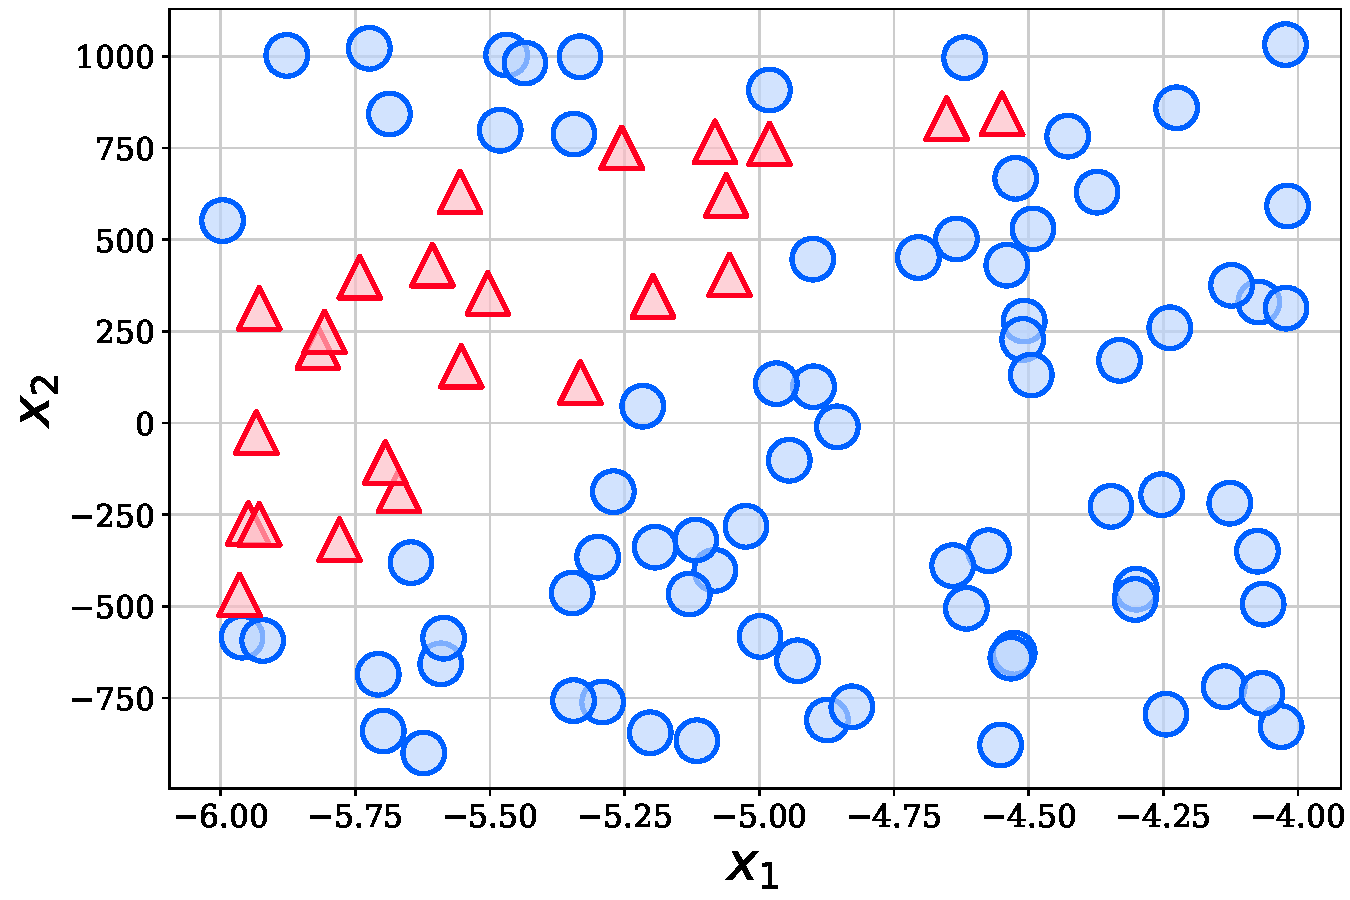
\includegraphics[width=0.9\textwidth]{figures/q1.pdf}
  \caption{The input data showing two types of observations with circles and triangles. Plotting code: \url{https://github.com/evgenyneu/ASP5020_data_analysis_problem_sets/blob/master/ps5/code/q1.py}.}
  \label{q1_two_observations}
\end{figure}

The diagram of the neural network is shown on \autoref{q1_network_diagram}. I choose the sigmoid activation function for the hidden layer nodes, because it's a common one in use. I will see how it work and switch to \emph{tanh} or \emph{ReLU} if needed. This is a classification task with just a single binary output (0 or 1). Therefore, for simplicity, I chose a single output node with no activation function (i.e. $f(x) = x$). If there were more than one output nodes than I could try a softmax function, but I will start simple and see how it goes.

\begin{figure}[!ht]
  \centering
  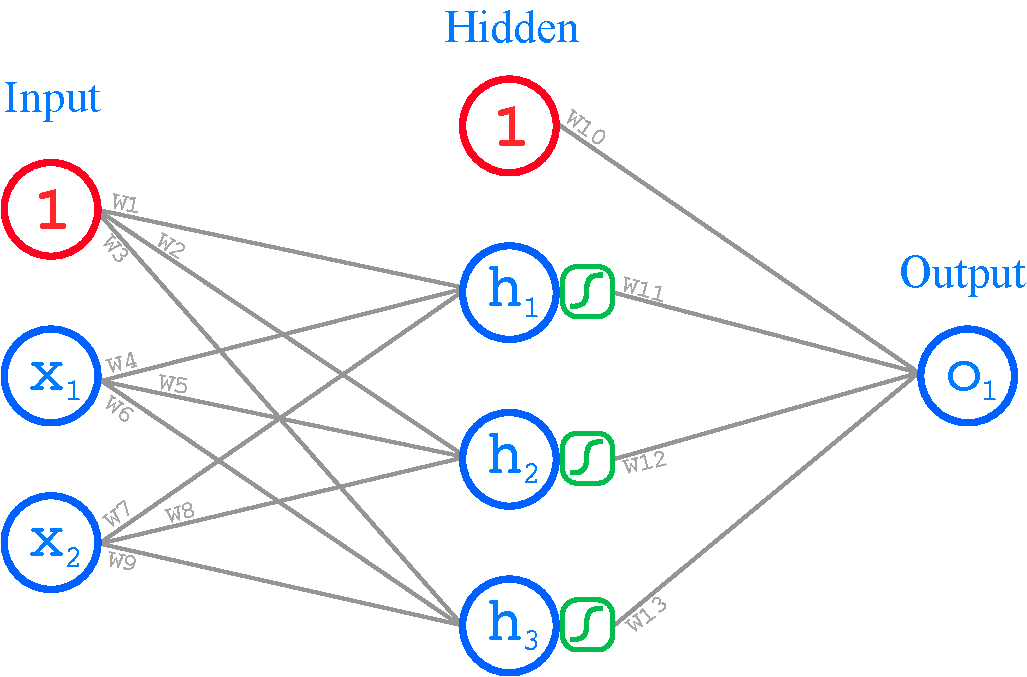
\includegraphics[width=0.7\textwidth]{figures/q1_neural_network.pdf}
  \caption{Diagram of the neural network containing two inputs ($x_1$ and $x_2$), single hidden layer with three nodes ($h_1$, $h_2$ and $h_3$) and a single output layer ($o_1$). The red circles with $1$ correspond to biases. Hidden layer nodes use sigmoid activation function. The labels $w1$ through $w13$ corredpond to the weight values, which are initialized by drawing random numbers from normal distribution $N(0, 1)$. Image source: \url{https://github.com/evgenyneu/ASP5020_data_analysis_problem_sets/blob/master/ps5/report/figures/q1_neural_network.sketch}}
  \label{q1_network_diagram}
\end{figure}


\subsection*{Removing sigmoid from output layer}

I do not use the sigmoid activation function in the output neuron because of the problem I found in the the Lecture 13 example code (\url{http://astrowizici.st/teaching/phs5000/13/}). I modified the code and replaced the sigmoid with $f(x) = x$ function. This was done because the output of the sigmoid is between 0 and 1, and it is used as predicted value from our model. However, in the loss function, we are comparing the predicted values with real values, which fall outside the $[0, 1]$ range. Therefore, the predicted value can never, even in theory, match the data. This mismatch is shown on \autoref{q1_lecture13_loss_compare}, where I compare the loss function of the original and the modified models. We can see that the modified model converges faster. The loss function for the original model will never approach zero, even if we increase the number of interations because of the range difference between the sigmoid and the data. The comparison of real and predicted values for the two codes are shown on \autoref{q1_lecture13_data_prediction_compare}. We can see that the original model can not be used for generating predicted values, since its range is limited.

\begin{figure}[!ht]
  \centering
  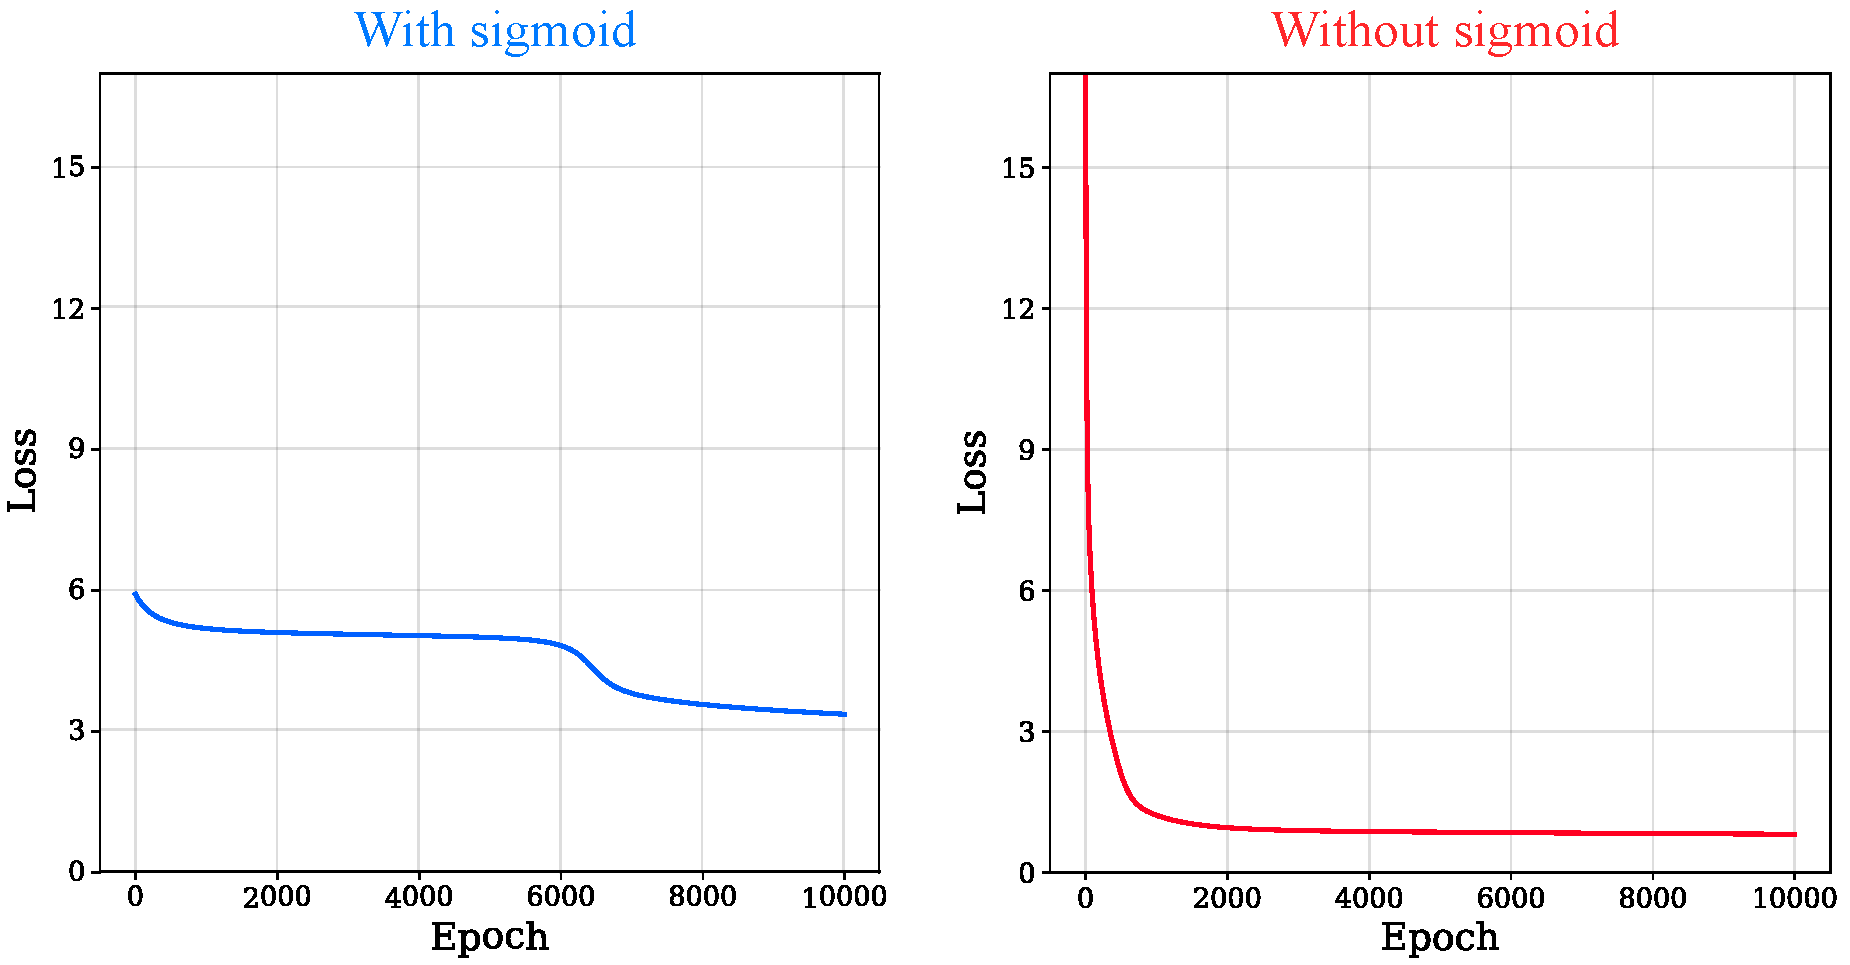
\includegraphics[width=1\textwidth]{figures/lecture13_loss_compared.pdf}
  \caption{Loss function for neural network from Lecture 13. The original code (left) contains sigmoid activation function in the output node, while the modified code (right) has no activation function ($f(x) = x$). Both codes are otherwise identical, including the same seeding of random number generators. The loss function of the original code (left) converges more slowly and never approaches zero. This is caused by mismatch between the range $[0, 1]$ of the sigmoid function and the data values, which are normalized to zero mean and standard deviation of 1.}
  \label{q1_lecture13_loss_compare}
\end{figure}


\begin{figure}[!ht]
  \centering
  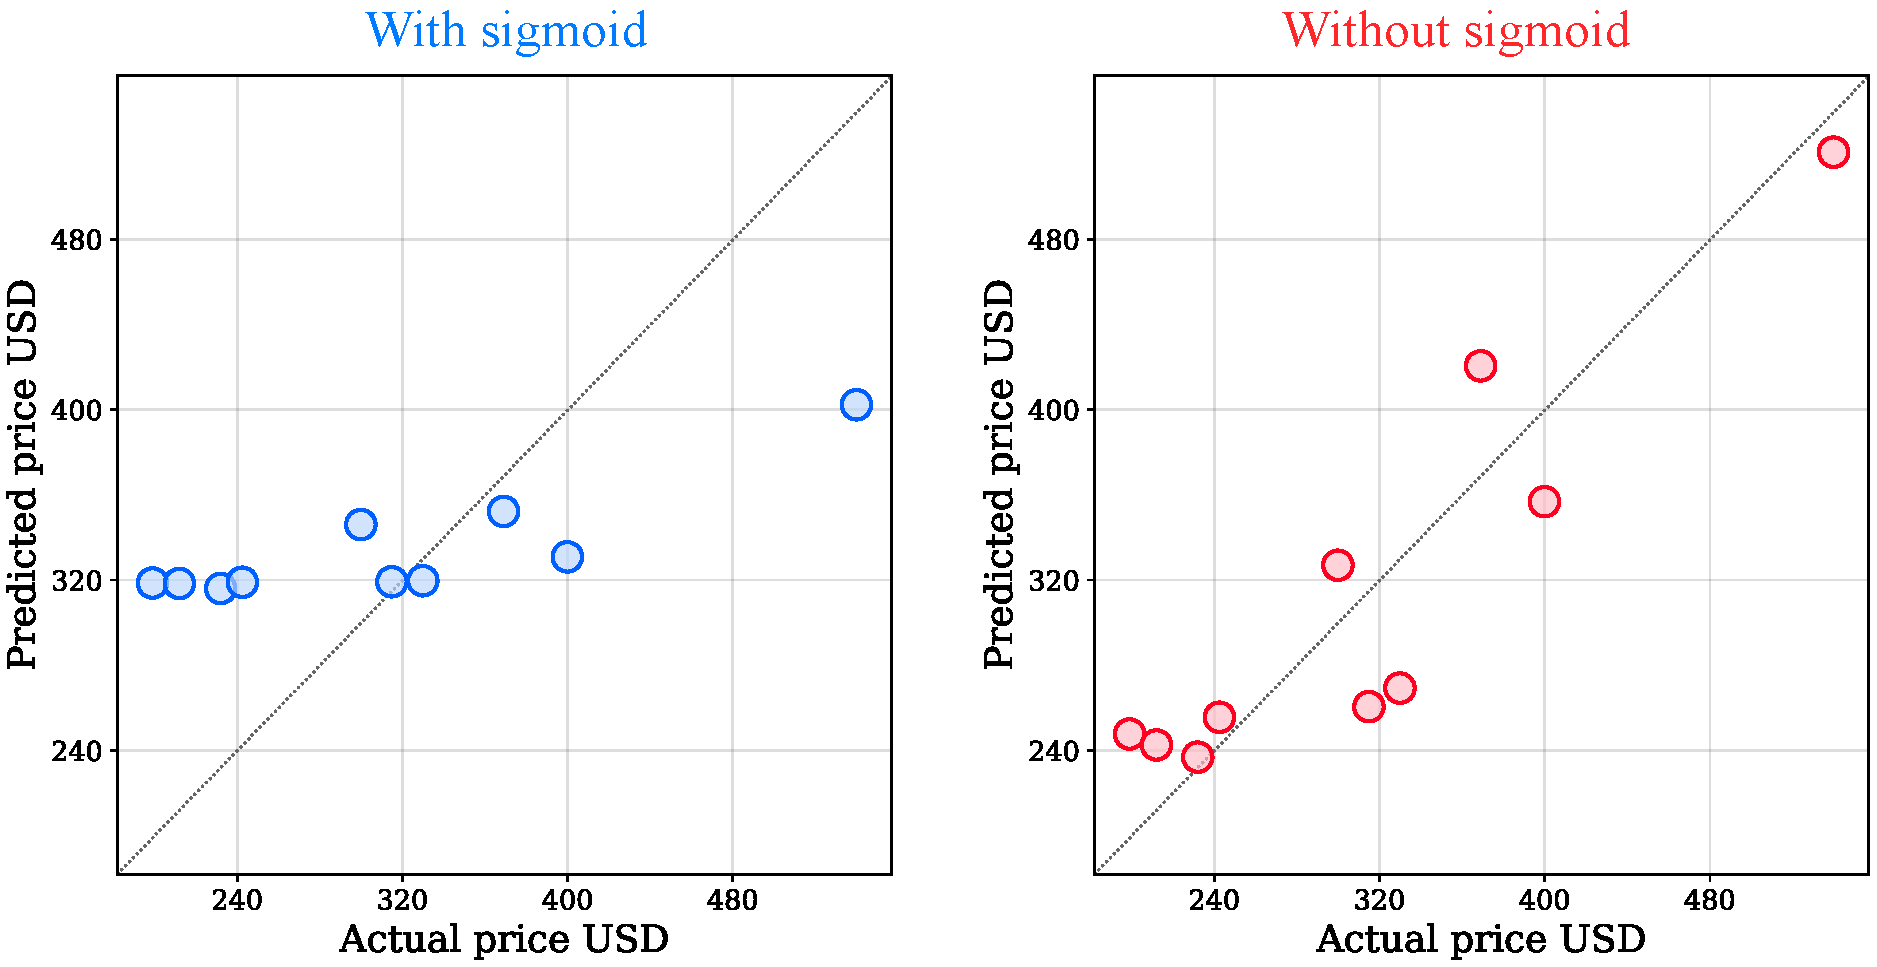
\includegraphics[width=1\textwidth]{figures/lecture13_results_compared.pdf}
  \caption{Comparison of model prediction (y axis) with data (x axis) for neural network code from Lecture 13. The original code (left) performs worse because because it's output range is limited to $[0, 1]$ multiplied by standard deviation and added mean of the data.}
  \label{q1_lecture13_data_prediction_compare}
\end{figure}



Original code form the lecture notes: \\ \url{https://github.com/evgenyneu/ASP5020_data_analysis_problem_sets/blob/master/ps5/code/lecture13_original_with_signoid_output.py}

My modified code without the output sigmoid (changed lines 99, 140 and 153): \\ \url{https://github.com/evgenyneu/ASP5020_data_analysis_problem_sets/blob/master/ps5/code/lecture13_remove_sigmoid_from_output.py}

The code changes are shown on \autoref{q1_lecture13_removing_loss_function}.


\begin{figure}[!ht]
  \centering
  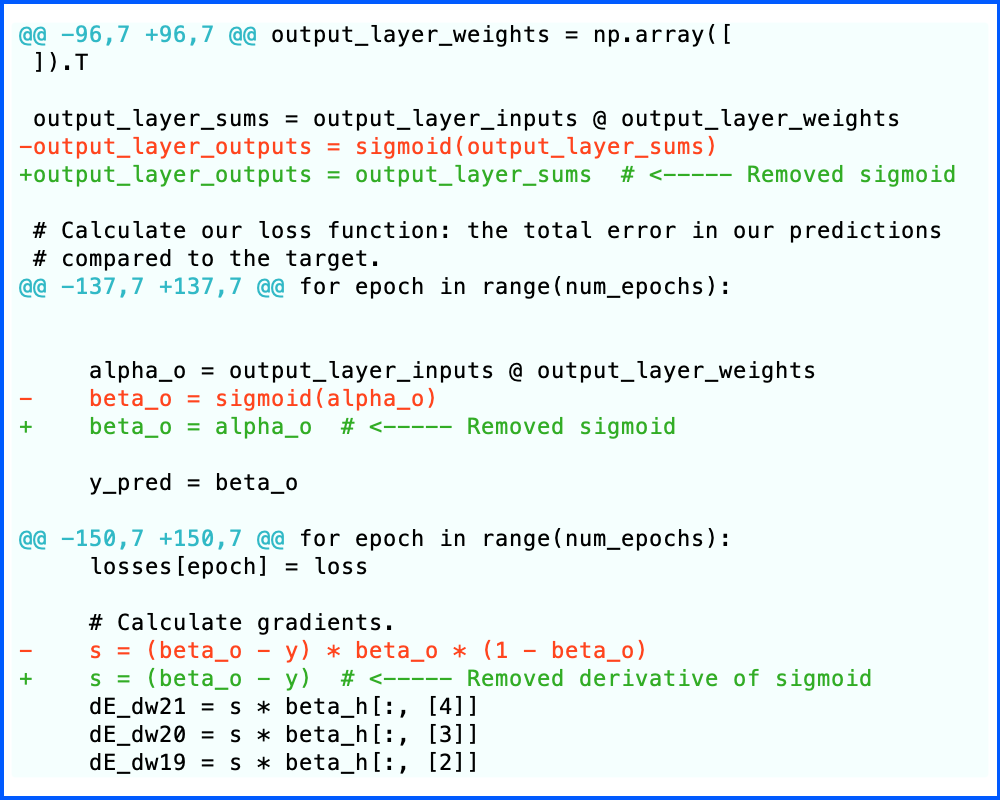
\includegraphics[width=0.8\textwidth]{figures/q1_lecture13_code_changes.png}
  \caption{Code changes that show removal of the sigmoid activation function from the output node.}
  \label{q1_lecture13_removing_loss_function}
\end{figure}







